% standalone wrapper for a tikz picture
\documentclass[tikz,border=2pt]{standalone}
\usepackage{xcolor}
\usepackage{tikz}
\usetikzlibrary{shapes,arrows,positioning,shadows,patterns,arrows.meta,calc}
\definecolor{cwAlert}{RGB}{220,50,50}
\definecolor{cwFlow}{RGB}{50,120,220}
\definecolor{cwDecoy}{RGB}{120,180,50}
\definecolor{cwBorder}{RGB}{80,80,80}
\definecolor{ImperialBlue}{RGB}{0,62,116}
\definecolor{ImperialNavy}{RGB}{0,33,71}
\definecolor{ImperialLightBlue}{RGB}{155,203,235}
\begin{document}

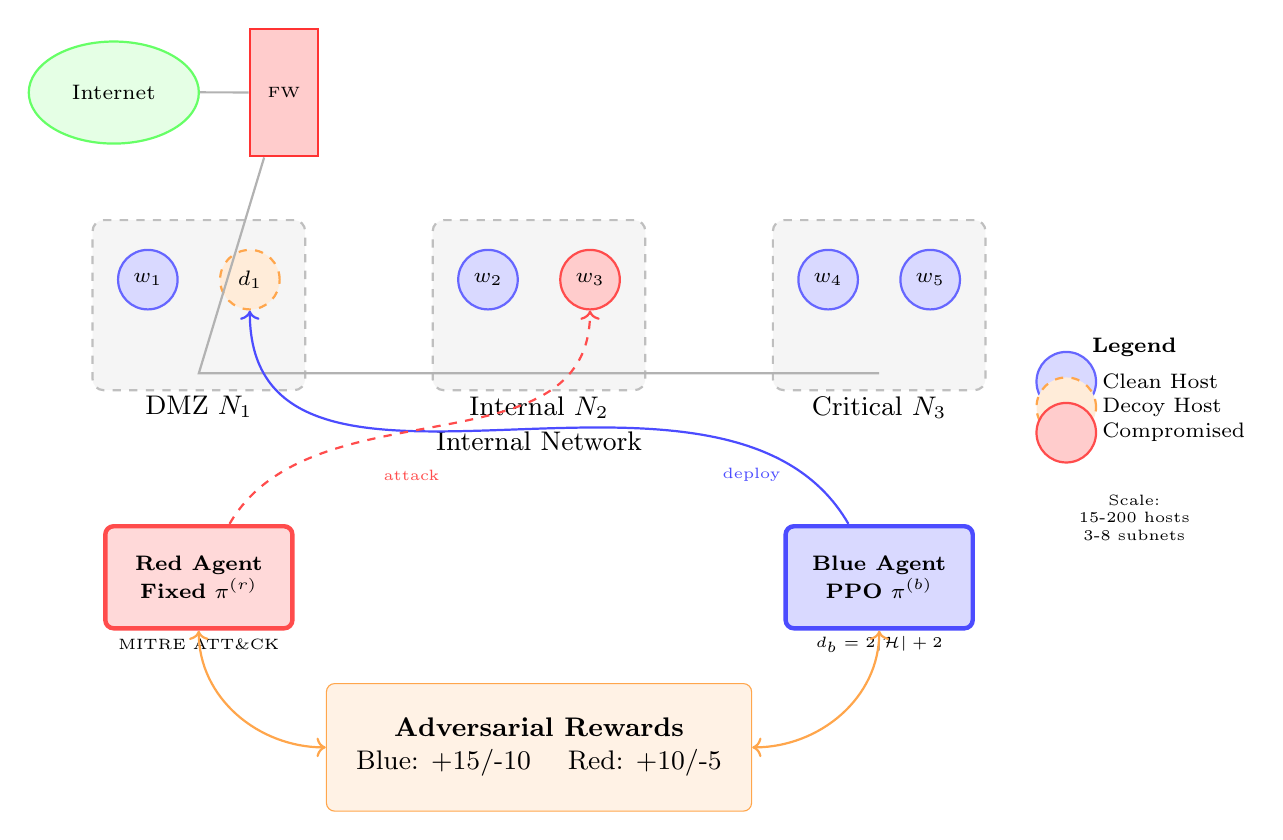
\begin{tikzpicture}[scale=1.08,transform shape,
    host/.style={circle, draw=blue!60, fill=blue!15, minimum size=7mm, font=\scriptsize, thick},
    decoy/.style={circle, draw=orange!70, fill=orange!15, minimum size=7mm, font=\scriptsize, thick, dashed},
    compromised/.style={circle, draw=red!70, fill=red!20, minimum size=7mm, font=\scriptsize, thick},
    subnet/.style={rectangle, draw=gray!50, fill=gray!8, minimum width=25mm, minimum height=20mm, thick, rounded corners=4pt, dashed},
    agentRed/.style={rectangle, draw=red!70, fill=red!15, minimum width=22mm, minimum height=12mm, font=\scriptsize, ultra thick, rounded corners=3pt},
    agentBlue/.style={rectangle, draw=blue!70, fill=blue!15, minimum width=22mm, minimum height=12mm, font=\scriptsize, ultra thick, rounded corners=3pt},
    firewall/.style={rectangle, draw=red!80, fill=red!20, minimum width=8mm, minimum height=15mm, font=\tiny, thick},
    internet/.style={ellipse, draw=green!60, fill=green!10, minimum width=20mm, minimum height=12mm, thick, align=center, font=\scriptsize}
]

% Internet - top left
\node[internet] (internet) at (-6, 6.5) {Internet};

% Firewall
\node[firewall] (firewall) at (-4, 6.5) {FW};

% Subnets - better spacing to avoid overlaps
\node[subnet] (subnet1) at (-5, 4) {};
\node[subnet] (subnet2) at (-1, 4) {};
\node[subnet] (subnet3) at (3, 4) {};

% Subnet labels - positioned clearly below subnets
\node[font=\small] at (-5, 2.8) {DMZ $N_1$};
\node[font=\small] at (-1, 2.8) {Internal $N_2$};
\node[font=\small] at (3, 2.8) {Critical $N_3$};

% Hosts - properly positioned within subnets
\node[host] (h1) at (-5.6, 4.3) {$w_1$};
\node[decoy] (d1) at (-4.4, 4.3) {$d_1$};

\node[host] (h2) at (-1.6, 4.3) {$w_2$};
\node[compromised] (h3) at (-0.4, 4.3) {$w_3$};

\node[host] (h4) at (2.4, 4.3) {$w_4$};
\node[host] (h5) at (3.6, 4.3) {$w_5$};

% Network backbone - adjusted positioning
\draw[thick, gray!60] (internet) -- (firewall);
\draw[thick, gray!60] (firewall) -- (-5, 3.2) -- (-1, 3.2) -- (3, 3.2);

% Internal Network label - positioned to avoid subnet overlap
\node[font=\small] at (-1, 2.4) {Internal Network};

% Agents - positioned lower to avoid overlap
\node[agentRed, align=center] (red) at (-5, 0.8) {\textbf{Red Agent}\\\textbf{Fixed} $\pi^{(r)}$};
\node[agentBlue, align=center] (blue) at (3, 0.8) {\textbf{Blue Agent}\\\textbf{PPO} $\pi^{(b)}$};

% Interactions with better label positioning
\draw[->, thick, blue!70] (blue) to[out=120, in=270] (d1);
\node[font=\tiny, blue!70] at (1.5, 2) {deploy};

\draw[->, thick, red!70, dashed] (red) to[out=60, in=270] (h3);
\node[font=\tiny, red!70] at (-2.5, 2) {attack};

% Essential state info
\node[font=\tiny] at (-5, 0.01) {MITRE ATT\&CK};
\node[font=\tiny] at (3, 0.01) {$d_b = 2|\mathcal{H}| + 2$};

% Rewards - positioned lower
\node[rectangle, draw=orange!70, fill=orange!10, minimum width=50mm, minimum height=15mm, rounded corners=3pt] (reward) at (-1, -1.2) {};
\node[font=\small, align=center] at (reward.center) {\textbf{Adversarial Rewards}\\Blue: +15/-10 \quad Red: +10/-5};

% Reward arrows
\draw[<->, orange!70, thick] (red.south) to[out=270, in=180] (reward.west);
\draw[<->, orange!70, thick] (blue.south) to[out=270, in=0] (reward.east);

\node[font=\scriptsize] at (6, 3.5) {\textbf{Legend}};
\node[host] at (5.2, 3.1) {}; \node[right, font=\scriptsize] at (5.5, 3.1) {Clean Host};
\node[decoy] at (5.2, 2.8) {}; \node[right, font=\scriptsize] at (5.5, 2.8) {Decoy Host};
\node[compromised] at (5.2, 2.5) {}; \node[right, font=\scriptsize] at (5.5, 2.5) {Compromised};

% Environment scale
\node[font=\tiny, align=center] at (6, 1.5) {Scale:\\15-200 hosts\\3-8 subnets};

\end{tikzpicture}
\end{document}
